\documentclass[11pt,
  titlepage=false,
  parskip=half,      % enable if you want paragraphs separated by vertical spacing instead of indents
]{scrreprt}

% Style settings
\usepackage[utf8]{inputenc}
\usepackage{microtype}
\usepackage[T1]{fontenc}
\usepackage{lmodern}
\usepackage{siunitx}
\usepackage{makecell}
\addtokomafont{disposition}{\rmfamily}

\usepackage[bsc,             % for Bachelor's Thesis titlepage
%project,        % for Master's Project titlepage
    claim,iaik]{iaikthesis}

\makeatletter\patchcmd{\scr@startchapter}{\if@openright\cleardoublepage\else\clearpage\fi}{}{}{}\makeatother

% Useful packages for complex content:
\usepackage{amsmath,amsfonts,amssymb} % typesetting math
%\usepackage{siunitx}                 % typesetting SI-units and formatted numbers
%\usepackage{listings}                % typesetting source code
\usepackage{booktabs,multirow}        % utils for complex/beautiful tables
\usepackage{subcaption}              % placing multiple subfigures in a figure
%\usepackage{graphicx}                % including external image files
%\usepackage{tikz}                    % drawing figures within LaTeX

% Bibliography, referencing, and indexing
\usepackage{csquotes}                 % typesetting \enquote{text in quotes} correctly
\usepackage[backend=biber,
            style=alphabetic,
            minalphanames=3, maxalphanames=4,
            maxbibnames=20]{biblatex} % to generate the bibliography
\addbibresource{report.bib}           % name of the bib-file

% Useful utils:
%\usepackage{todonotes}               % add ToDo markers (\todo{...}, \todo[inline]{...})
\usepackage[hidelinks]{hyperref}
\usepackage{textcomp}
\usepackage{graphicx}
\usepackage{listings}      % clickable links (but hide color frames around links)
%\usepackage{cleveref}                % named references (\Cref{chap:introduction}, ...)

% Your own macros:
%\newcommand{\mynewmacro}[1]{my content with one input parameter: #1}


\usepackage{color}
\definecolor{lightgray}{rgb}{.9,.9,.9}
\definecolor{darkgray}{rgb}{.4,.4,.4}
\definecolor{purple}{rgb}{0.65, 0.12, 0.82}
\lstdefinelanguage{JavaScript}{
  keywords={break, case, catch, continue, debugger, default, delete, do, else, false, finally, for, function, if, in, instanceof, new, null, return, switch, this, throw, true, try, typeof, var, void, while, with},
  morecomment=[l]{//},
  morecomment=[s]{/*}{*/},
  morestring=[b]',
  morestring=[b]",
  ndkeywords={class, export, boolean, throw, implements, import, this},
  keywordstyle=\color{blue}\bfseries,
  ndkeywordstyle=\color{darkgray}\bfseries,
  identifierstyle=\color{black},
  commentstyle=\color{purple}\ttfamily,
  stringstyle=\color{red}\ttfamily,
  sensitive=true,
}

\lstset{
   language=JavaScript,
   backgroundcolor=\color{white},
   extendedchars=true,
   basicstyle=\footnotesize\ttfamily,
   showstringspaces=false,
   showspaces=false,
   numbers=left,
   numberstyle=\footnotesize,
   numbersep=9pt,
   tabsize=2,
   breaklines=true,
   showtabs=false,
   captionpos=b,
   frame=single,
}

\begin{document}

%--- FRONT MATTER --------------------------------------------------------------

%--- INSERT INFORMATION FOR TITLEPAGE ------------------------------------------

% Your name + previous academic degrees:
\thesisauthor{Christoph Royer}

% Title of your thesis:
\thesistitle{JavaSQUIP\\Implementing a scheduler queue-based covert channel in JavaScript}

% Date of completion:
\thesisdate{October 2024}

% Supervisor:
\supervisortitle{}
\supervisor{
    \textbf{Advisor}: Stefan Gast\\
    \textbf{Supervisor}: Daniel Gruss
    \smallskip

    Institute of Applied Information Processing and Communications\\
    Graz University of Technology
}

% Name of your degree programme according to your curriculum
\curriculum{Computer Science}

\printthesistitle

\chapter*{\centering\Large Abstract}
\label{ch:abstract}
The implementation of out-of-order execution has brought a big performance benefit to current CPUs.
With this benefit also come security concerns however, since attackers can exploit the timing variations which are bound to occur in an out-of-order pipeline.
Attacks which target only one execution unit through a separate scheduler queue -- as seen in the Apple M1 and AMD Zen 3 and Zen 4 microarchitectures -- have proven even more powerful than port contention on single-scheduler systems.
As with any attack, porting this side channel to the web would greatly increase its reach and number of victims.

In this thesis, we present the JavaSQUIP attack, which is a port of SQUIP~\cite{squip} to JavaScript.
We look into the security measures used in common browsers to prevent timing attacks, and show how we worked around them successfully.

Our covert channel can provide communication across separate browser instances at a speed of 1000 bits/s,
which is faster than any current covert channel of this type.
At this speed, we are able to achieve a transmission accuracy of $99.2~\%$ and $99.3~\%$ on Zen 3 and Zen 4 respectively.

Modern CPUs are becoming ever more complex, and with this complexity come more possibilities for side channel attacks.
JavaSQUIP makes it clear that the security measures of current browsers have not yet adapted to protect against these kinds of attacks.
Our findings suggest that making these attacks impossible may not even be feasible because the drawbacks in performance and features would be too extensive.
\paragraph{Keywords:}
Covert channel $\cdot$
Scheduler queue contention $\cdot$
JavaScript $\cdot$
AMD Zen

\clearpage

%--- INTRODUCTION --------------------------------------------------------------

\chapter{Introduction}
\label{ch:introduction}

Nowadays, CPU manufacturers are in a steady competition against each other to make their products faster and faster.
One of the ways this is achieved is \textit{out-of-order execution}, where instructions are not executed in program order,
but rather as soon as their respective dependencies are ready and a suitable execution unit is free.
Although this toes the line of breaking the hardware-software contract, the CPU ensures that out-of-order execution remains transparent to the user.
To better balance usage of its execution units, modern CPUs often also include \textit{Simultaneous Multithreading} (SMT).
Here, one physical core is split up into two logical cores, which share physical infrastructure like the schedulers and execution units.

Out-of-order execution and SMT are designed to be transparent to the user, however attacks like
PortSmash~\cite{Aldaya2019port} and SMoTherSpectre~\cite{Bhattacharyya2019} show that combining the two technologies presents a viable attack surface.
By measuring timing variations in out-of-order execution, an attacker can gain insight into sensitive information.
This attack, which targets all CPUs with SMT, is called \textit{port contention}.
%Because the instructions are reordered on the fly, the CPUs scheduler needs to distribute incoming instructions across the ports for its several specialized execution units.
If the attacker is co-located with the victim on the same core, they can measure delays when issuing instructions to a shared execution unit.
In this way, the attacker can gain knowledge on the victim's execution based on whether instructions are delayed by the scheduler or not.

SQUIP~\cite{squip} focuses on CPUs with multiple specialized scheduler queues to implement \textit{scheduler queue contention}.
Each scheduler deals with fewer execution units, which is why the attacker can push one of the comparatively small scheduler queues close to its capacity.
If the victim also adds to the queue, the pipeline stalls, which results in a significant increase in execution time.
This makes SQUIP a fast and reliable covert channel on many modern CPU architectures such as the AMD Zen 3.~\cite{squip}

Since implementations of port contention-based side channels in a browser setting already exist~\cite{Rokicki2022webport}, we ask the following research questions:

\textit{
    Can per-execution-unit scheduler queue contention be exploited in a browser setting?
    Are there significant benefits compared to single scheduler port contention-based approaches?
}

\pagebreak
\paragraph{Contributions.}
In this thesis, we contribute the following:
\begin{itemize}
    \item We present JavaSQUIP, a browser-based covert channel based on the SQUIP~\cite{squip} attack.
    \item We show that JavaSQUIP is reliable and faster than approaches based on CPU architectures with a single scheduler queue.
    \item We develop a framework for transmitting data between separate instances of a browser at speeds of up to 1000 bit/s.
    \item We argue that JavaSQUIP relies on essential features of JavaScript, meaning the threat it poses cannot be easily mitigated.
\end{itemize}

\paragraph{Outline.}
In Section~\ref{ch:background}, we provide relevant background information on scheduler queue contention,
resulting in several challenges that we will have to overcome when implementing JavaSQUIP.
Section~\ref{ch:implementation} shows how we dealt with these challenges.
Section~\ref{ch:optimisation} continues by explaining how we optimised JavaSQUIP for speed and reliability.
We go into more detail on the mode and results of our evaluation of JavaSQUIP in Section~\ref{ch:evaluation}.
In Section~\ref{ch:comparison}, we present comparable covert channels and compare them to JavaSQUIP.
We propose ways to prevent JavaSQUIP in Section~\ref{ch:countermeasures} and discuss whether they are feasible.
We conclude with Section~\ref{ch:conclusion}, outlining potential use cases and discussing the implications of the attack.


%--- BACKGROUND ----------------------------------------------------------------
\chapter{Background}
\label{ch:background}

In this chapter, we go into detail on two aspects of CPU scheduling
-- \textit{Out-Of-Order Execution} and \textit{Simultaneous Multithreading} --
and how they have been exploited by prior work.
Furthermore, we take a closer look into the browser features needed to implement these exploits in JavaScript.

\section{Out-Of-Order Execution}
\label{sec:outoforderexecution}
For performance reasons, modern CPUs use efficiency features at almost every stage of an instruction's execution.
One notable feature is \textit{Out-Of-Order Execution},
where instructions are split up into smaller parts.
These so-called \textit{\textmu ops} can be executed in a diffent order than the program order,
enabling a more efficient utilisation of the CPU's resources.

The following paragraphs describe the stages of an instruction in a CISC CPU,
where Out-Of-Order Execution is utilised.

\paragraph{Fetch.}
Before an instruction can be executed, it needs to be loaded from cache or memory.
As branches can make loading unpredictable and loading the wrong instruction is expensive, a \textit{branch prediction unit} tries to guess which path is more likely to be loaded.
Taking this one step further, the predicted path may also be executed before the condition for the branch has been computed.
This is called \textit{speculative execution}~\cite{AMD2020OptimizationEPYC7002}.

% TODO: Are there attacks against the decoder too?
\paragraph{Decode.}
Modern CISC CPUs divide complex instructions into their parts when possible;
these parts are called \textit{micro-ops} (\textmu ops)~\cite{AMD2020OptimizationEPYC7002}.
For example, an addition with memory operands may be split up into three \textmu ops: one for loading the operands, one for the addition, and one for storing the result.
These \textmu ops can be distributed across specialized execution units, enabling more parallelization and load balancing, and thus an increase in performance.

\begin{figure}
    \centering
    \begin{subfigure}[b]{\textwidth}
        \centering
        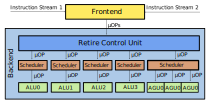
\includegraphics[width=0.7\textwidth]{figures/Zen2 arch}
        \caption{The scheduler layout in AMD Zen~2 (c.f.~\cite{AMD2020OptimizationEPYC7002})}
        \label{fig:amdzen2}
    \end{subfigure}

    \begin{subfigure}[b]{\textwidth}
        \centering
        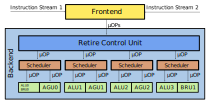
\includegraphics[width=0.7\textwidth]{figures/Zen3 arch}
        \caption{The scheduler layout in AMD Zen~3 (c.f.~\cite{AMD2020OptimizationEPYC7003})}
        \label{fig:amdzen3}
    \end{subfigure}
    \caption{Comparison of the scheduler layouts of AMD Zen~2~and~3 architectures}
    \label{fig:amdzencomparison}
\end{figure}

\paragraph{Schedule/Execute.}
Once created, the \textmu ops are queued to be executed as soon as their dependencies are met -- sometimes out of the order of their arrival.
Depending on the CPU microarchitecture, there can be one general scheduler queue for all execution units, or multiple.
While Intel uses one scheduler queue for all its execution units~\cite{Intel_opt},
architectures like AMD's Zen~2~\cite{AMD2020OptimizationEPYC7002}, Zen~3~\cite{AMD2020OptimizationEPYC7003} and Zen~4~\cite{AMD2023OptimizationZen4} use several specialized scheduler queues.
When multiple scheduler queues are used, different queues can be specialized for a specific \textmu op or class of \textmu ops.
Figure~\ref{fig:amdzencomparison} illustrates the concept.
Splitting the scheduler queue reduces complexity and enables more efficient power usage.



\paragraph{Retire.}
After all the \textmu ops of an instruction have completed, the \textit{retire control unit} (RCU) reassembles the results.
It commits the finished instructions and schedules dependent instructions -- the dissection into \textmu ops is transparent to the user.

\section{Simultaneous Multithreading}
\label{sec:smt}

As we described in more detail in Chapter~\ref{sec:outoforderexecution},
the cores of a modern CPU are subdivided into multiple specialized execution units.
If only one thread would be executed on such a core,
most of these execution units would stay unused while an instruction is executed.

With \textit{Simultaneous Multithreading} (SMT), one physical core is split into multiple logical cores
-- most commonly, two logical cores per physical core are implemented~\cite{tullsen1995simultaneous}.
This means that one core executes two threads simultaneously, distributing the workload across its execution units more effectively.
Tests show that this provides an average performance gain of about $25~\%$~\cite{Phoronix2018HT, Cutress2020SMT}
with relatively little additional architecture needed.

The two threads that are being executed on the same core are called \textit{co-located}.
Usually, these threads should be unaffected by each other; no data is exchanged between two co-located threads.
However, the sharing of common architecture, particularly the execution units, enables several different side channels.
All of them are \textit{timing attacks}, meaning that they gain information by measuring execution times of a piece of code.
A selection of these attacks will be explained in the following chapter.

\section{Prior attacks on the CPU pipeline }
\label{sec:exploits}
Many of the stages of an instruction's life cycle are exploitable;
in the following, we will list some of the exploits that have already been found.

\paragraph{Speculative Execution.}
Executing a path before the condition for the branch is known --
can be exploited, as was shown by Spectre~\cite{spKocherHFGGHHLM019}.

First, the branch prediction unit is primed by repeatedly branching with the condition set to \textit{A}.
In the second step, the branch is called again, but with the condition set to \textit{B}.

Since the branch prediction unit was trained to expect condition \textit{A},
the CPU can be tricked into executing an inaccessible path.
Under the right circumstances, this can be used to leak data from a co-located process.

\paragraph{Port Contention.}
PortSmash~\cite{Aldaya2019port} and SMoTherSpectre~\cite{Bhattacharyya2019} exploit port contention.
They use the fact that only one of the two threads in an SMT-enabled core can use an execution unit in a single cycle.
The attacker can thus find out whether the victim is using a port by measuring the execution time of an instruction on the same port.
Delayed execution gives away the fact that the victim is currently using that port.
Port contention works independently of the type of scheduler queue used.
It affects only one execution unit, and thus creates contention and measures execution time with the same instruction.

\begin{figure}
    \begin{subfigure}[b]{\textwidth}
        \centering
        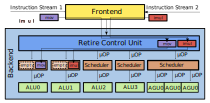
\includegraphics[width=0.7\textwidth]{figures/Zen2 normal operation}
        \caption{An AMD Zen~2 processor in normal operation: the two instruction streams do not impede each other}
        \label{fig:amdzen2normaloperation}
    \end{subfigure}

    \begin{subfigure}[b]{\textwidth}
        \centering
        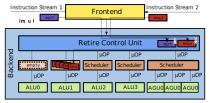
\includegraphics[width=0.7\textwidth]{figures/Zen2 sqc}
        \caption{An AMD Zen~2 processor exhibiting scheduler queue contention: a stall on the Scheduler queue for ALU1 stalls both instruction streams}
        \label{fig:amdzen2sqc}
    \end{subfigure}

    \caption{Comparison between normal operation and scheduler queue contention in an AMD Zen~2 Processor}
    \label{fig:amdzen2normalvssqc}
\end{figure}

\paragraph{Scheduler Queue Contention.}
SQUIP~\cite{squip} on the other hand exploits scheduler queue contention.
In scheduler queue contention, the attacker fills up the scheduler queue to the point that it is almost at its capacity limit;
any activity of the victim that involves this scheduler queue will overflow the queue, leading to a queue stall.
A queue stall occurs when more \textmu ops of a particular type are created than what the correlating scheduler queue can hold.
Because the CPU cannot drop any \textmu ops, it has to stall the loading of new instructions entirely until the scheduler queue is free again.
The attacker can measure this easily because it entails a significant increase in execution time --
not only for instructions in the affected queue, but on the whole core.
Figure~\ref{fig:amdzen2sqc} shows how one instruction stream can stall the other just by filling up the relatively small scheduler queue.


SQUIP is limited in its applicable CPU architectures because it relies on the split-scheduler architecture of AMD Zen~2, Zen~3 and Zen~4 CPUs to distinguish between \textmu ops.
However, its advantage is a higher transmission rate compared to port contention.
Because scheduler queue contention stalls the whole CPU, as compared to port contention stalling just one execution unit,
a comparatively bigger increase in execution time is achieved.
SQUIP produces stalls with instructions on a different execution unit than the unit where execution time is measured (see Figure~\ref{fig:amdzen2sqc}).
The measured execution unit either sees low load -- the measurement instructions, or a complete stall -- scheduler queue contention,
as illustrated in Figure~\ref{fig:amdzen2normalvssqc}.
%Additionally, SQUIP creates very few instuctions on the execution unit where execution times are measured,
%since stalls are produced on another unit.
%This means that the measured execution unit goes from low load to being stalled completely (see Figure~\ref{fig:amdzen2normalvssqc}).
This increases the signal-to-noise ratio of the timing measurement,
enabling shorter time slices per bit.
All of this gives SQUIP~\cite{squip} higher potential transmission speeds and reliability than port-contention based side channels.
Because of this advantage, JavaSQUIP aims to port this vulnerability to a browser environment.

\section{JavaScript in a browser environment}
\label{sec:javascriptenv}
JavaScript~\cite{javascript} is the main scripting language for running code in a website.
It is an interpreted language, which means that the browser executes code without compilation into a binary format.
JavaScript developers benefit from writing high-level platform-independent code,
while the interpreter takes care of executing it on the user's machine.

To improve performance, modern browsers use \textit{just-in-time (JIT) compilation}~\cite{jitcompiler}.
The interpreter monitors the program flow during execution.
If a function is called very often,
it is computationally cheaper to compile it once rather than repeatedly interpreting it.
The compilation is done in two stages: baseline compilation and optimized compilation.
The baseline compiler creates the binary representation of the function.
It also optimizes away unnecessary code, such as unused calculations, while keeping the execution equivalent to the script.
If the function is repeatedly called with similar arguments, the optimized compiler creates a second binary code.
This second binary is optimized based on assumptions about the arguments -- such as their types and properties.
The optimized binary is executed after assessing the truth of the assumptions, and is discarded if the assumptions do not hold.

\section{Browser security measures}
\label{sec:browsersecurity}
% todo these citations ugly
Since the advent of many timing side and covert channels~\cite{noack2018exploiting, Rokicki2022webport, gruss2016rowhammer, 185126},
browser developers have implemented many measures to mitigate the threat~\cite{shusterman2021prime, performancenow, performancenowchrome, schwarz2018javascript}.
This has always meant striking a balance between security and efficiency.
Because of this, many potential attack surfaces cannot be eliminated without unreasonable losses in performance and functionality,
though some measures do slow down side and covert channels significantly.

In the following we expand on security measures regarding multithreading, accurate timing in browsers, and low-level operations.
All three of these are needed to mount the SQUIP attack.


\subsection{Timing functions}\label{subsec:timingjs}
There are two contenders for timing measurements in JavaScript: \texttt{Date.now()}~\cite{datenow} and \texttt{performance.now()}~\cite{performancenow}.

The \texttt{Date.now()}~\cite{datenow} function gives a synchronised Unix epoch timestamp with millisecond accuracy.
The Unix epoch time is essentially the time elapsed since January 1, 1970 and is the same for all processes on a computer.
This makes \texttt{Date.now()} a cross-instance synchronised timestamp.

\texttt{performance.now()}~\cite{performancenow} measures the time elapsed since the \textit{time origin} of the current context.
This means that \texttt{performance.now()} gives different values between browser instances, and even between a main thread and its worker threads.
Timing information from \texttt{performance.now()} can still be synchronised;
The \textit{time origin} of the context is given by the \texttt{performance.timeOrigin()}~\cite{performancetimeorigin} property.
This way, the timestamps from \texttt{performance.now()} can be globally synchronised.

The accuracy of \texttt{performance.now()} has been heavily restricted by browser developers to counteract the threat of timing attacks.
For example, in Firefox it has an accuracy of 1 ms, and in Chrome it measures with an accuracy of 0.1 ms~\cite{performancenow, performancenowchrome}.

Consequently, both \texttt{Date.now()} and \texttt{performance.now()} give a synchronised timestamp with 1 ms accuracy, making them viable options for synchronisation.

\subsection{Multithreading}\label{subsec:multithreading}
JavaScript does not support low-level control over threading, but the \texttt{Web Workers} API~\cite{webworkers} allows the user to create workers running in a separate thread.
An instantiated worker runs a predefined script.
The main thread can interface with the worker via calls to the \texttt{Worker.postMessage()} function and via a \texttt{SharedArrayBuffer}~\cite{sharedarraybuffer}.
There is no support for selecting a core on which a worker is run on, presenting a challenge to co-locate with the sender.

Creating a \texttt{SharedArrayBuffer} is restricted in two ways: the browser window needs to be SSL-encrypted, and it needs to restrict some Cross-Origin requests.
Nevertheless, this is not a problem for an attacker on any site that provides \texttt{https} and where all code comes from a single origin.
With the help of free, easy-to-use ssl certificates such as certbot~\cite{certbot}, almost every website on the internet provides an SSL-encrypted connection.
This means that the requirements for a \texttt{SharedArrayBuffer} are likely to be met for any public website where a malicious actor would place their code.

%todo mention jit compiler
\subsection{Low-level operations in JavaScript}\label{subsec:lowleveljs}
To create contention on one specific scheduler queue, we need a way to create a stream of equal and co-dependent instructions -- specifically the \texttt{imul} instruction.
One way to achieve this in a browser context would be \textit{WebAssembly}~\cite{webassembly}.
For the sake of using as few features of the browser as possible, we implement the needed functionality in JavaScript.

JavaScript handles numbers as floating-point numbers by default.
This means that a simple invocation of a multiplication like \texttt{a * b;} in JavaScript will not result in an \texttt{imul} instruction on the CPU.
Rather, \texttt{Math.imul(a, b)}~\cite{mathimul} gives the user a lower-level command:
It interprets the parameters as 32~bit integers and multiplies them as such, resulting in an \texttt{imul} instruction on the CPU.
We verify which instructions were generated by running code through V8 -- the compiler used in Chrome --
using the JavaScript explorer on godbolt.org~\cite{godbolt}.
% todo but we use firefox/seamonkey
% https://blog.mozilla.org/attack-and-defense/2020/09/15/inspecting-just-in-time-compiled-javascript/

\begin{lstlisting}[float,caption={A test function for the \texttt{imul} instruction},label={lst:testimul},language=JavaScript]
function test(a) {
a = Math.imul(a, a);
a = Math.imul(a, a);
a = Math.imul(a, a);
a = Math.imul(a, a);
a = Math.imul(a, a);
return a;
}
\end{lstlisting}

\begin{lstlisting}[float,caption={The compiled result of the \texttt{imul} test function},label={lst:compileimul}]
0x6469d68040b8    78  0f80ba000000         jo 0x6469d6804178  <+0x138>
0x6469d68040be    7e  8bc9                 movl rcx,rcx
0x6469d68040c0    80  8bf9                 movl rdi,rcx
0x6469d68040c2    82  0faff9               imull rdi,rcx
0x6469d68040c5    85  8bcf                 movl rcx,rdi
0x6469d68040c7    87  0fafcf               imull rcx,rdi
0x6469d68040ca    8a  8bf9                 movl rdi,rcx
0x6469d68040cc    8c  0faff9               imull rdi,rcx
0x6469d68040cf    8f  8bcf                 movl rcx,rdi
0x6469d68040d1    91  0fafcf               imull rcx,rdi
0x6469d68040d4    94  8bf9                 movl rdi,rcx
0x6469d68040d6    96  0faff9               imull rdi,rcx
0x6469d68040d9    99  488bcf               REX.W movq rcx,rdi
0x6469d68040dc    9c  03cf                 addl rcx,rdi
0x6469d68040de    9e  0f8046000000         jo 0x6469d680412a  <+0xea>
\end{lstlisting}

\begin{lstlisting}[float,caption={A test function for the \texttt{sqrt} instruction},label={lst:testsqrt},language=JavaScript]
function test(a) {
a = Math.sqrt(a);
a = Math.sqrt(a);
a = Math.sqrt(a);
a = Math.sqrt(a);
a = Math.sqrt(a);
return a;
}
\end{lstlisting}

\begin{lstlisting}[float,caption={The compiled result of the \texttt{sqrt} test function},label={lst:compilesqrt}]
0x62a1e00040aa    6a  c5fb104103           vmovsd xmm0,[rcx+0x3]
0x62a1e00040af    6f  c5fb51c0             vsqrtsd xmm0,xmm0,xmm0
0x62a1e00040b3    73  c5fb51c0             vsqrtsd xmm0,xmm0,xmm0
0x62a1e00040b7    77  c5fb51c0             vsqrtsd xmm0,xmm0,xmm0
0x62a1e00040bb    7b  c5fb51c0             vsqrtsd xmm0,xmm0,xmm0
0x62a1e00040bf    7f  c5fb51c0             vsqrtsd xmm0,xmm0,xmm0
0x62a1e00040c3    83  c5fb2cc8             vcvttsd2si rcx,xmm0
0x62a1e00040c7    87  c5832ac9             vcvtlsi2sd xmm1,xmm15,rcx
0x62a1e00040cb    8b  c5f92ec8             vucomisd xmm1,xmm0
\end{lstlisting}

A test function in Listing~\ref{lst:testimul} contains multiple \texttt{Math.imul()} calls.
The resulting binary in Listing~\ref{lst:compileimul} contains the \texttt{imul} instruction.
Similarly, \texttt{Math.sqrt()}~\cite{mathsqrt} translates to the \texttt{sqrt} instruction (see Listing~\ref{lst:testsqrt} and Listing~\ref{lst:compilesqrt}).

%--- IMPLEMENTATION ----------------------------------------------------------------
\chapter{Implementing JavaSQUIP}
\label{ch:implementation}
As described in Section~\ref{sec:browsersecurity}, there are some challenges to overcome when implementing a timing attack in a browser.
This chapter explains how we work around these challenges to implement the JavaSQUIP covert channel.

\section{General architecture}
\label{sec:general-architecture}
We build a showcase for JavaSQUIP consisting of two web pages: one receiver and one sender.
The aim is to build a showcase that, while showing the capabilities of the covert channel,
should reflect as realistic a scenario as possible to also prove the feasibility of a side channel attack.
The difference between a conventional side channel attack and a covert channel is that a side channel attack involves a (non-cooperating) victim and
an attacker, while covert channels have a cooperating pair of sender and receiver.
% todo example of cooperation

The sender in the showcase corresponds to the victim in a side channel scenario.
Since a victim does not cooperate in an attack, the sender was kept as simple as possible.
It consists of one thread, sending one bit per timeslice (see \ref{sec:accurate-timing}) via issuing \texttt{Math.imul()} instructions or not.

The receiver represents the attacker.
The assumption is that an attacker can execute arbitrary scripts, for example as an interactive advertisement on a website.
Given this, the attacker can get one thread co-located with the victim and exploit the SQUIP side channel to gain information.
Details on the implementation are described in the following chapters.

\section{Getting accurate timing}
\label{sec:accurate-timing}
JavaSQUIP needs two kinds of timing in order to work properly:
\begin{itemize}
    \item a cross-process syncronized clock to determine the start of bit transmissions:\\
    resolution of ${f_{\text{transmission}}}^{-1} \approx$ 1ms
    \item a fine-grained measurement to measure port contention:\\
    resolution of 100 CPU cycles $\approx$ 25ns
\end{itemize}

For the synchronised clock, we can use \texttt{Date.now()}~\cite{datenow}, which has a 1ms accuracy.
This allows us to partition the duration of the transmission into 1ms \textit{timeslices}.
During one timeslice, a single bit can be transmitted by the existence or absence of scheduler queue contention.
The alignment of bytes is solved by starting the transmission on a multiple of 8 timeslices since the start of the epoch (see \ref{subsec:timingjs}).
Synchronising with \texttt{Date.now()}~\cite{datenow} works, but only for transmissions of up to 1000 bits/s,
since there is no more precise timestamp in JavaScript which is synchronised across browser instances.

%To get around this and realize a faster transmission than 1000 bits/s, we propose implementing the Manchester Code~\cite{manchesterEncoding}.
%It is self-synchronising, which eliminates the need for an external source of synchronisation.
%The actual implementation is not within the scope of this thesis.

The receiver also needs a way to measure the small variations in timing whenever a scheduler queue gets blocked.
Since no timing function in JavaScript gives a better accuracy than 0.1ms, we need to provide our own timing.

We solve this with a counting worker, which continually increases one variable in the \texttt{SharedArrayBuffer}.
As explained in section \ref{subsec:multithreading}, the other receiver workers can then access this counter and use it to measure execution times with adequate accuracy.
The paper on \textit{Fantastic Timers}~\cite{Schwarz2017Timers} explains the concept in more depth.
% todo code snippet of counting worker

\section{Co-locating with the sender}
\label{sec:co-location}

\begin{figure}
\centering
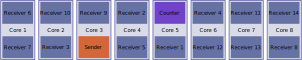
\includegraphics[width=\textwidth]{figures/colocation}

\caption{One possible co-location configuration. The counting thread is co-located with Receiver 1, the Sender is co-located with Receiver 9.}
\label{fig:colocation}

\end{figure}

JavaScript does not provide the functionality of binding to a particular core,
the receiver tries to force co-location by crowding the CPU.
The receiver has one thread running on each virtual core,
leaving just one virtual core open for the sender's thread to occupy.
To do this the receiver creates as many receiving workers as the number of virtual cores in the machine, minus two:
one for the counting thread (see \ref{sec:accurate-timing}), and one for the sending thread.
In our experiments, we use an \textit{AMD Ryzen 7 5800X} as representative for Zen~3 and an \textit{AMD Ryzen 7 7700X} as representative for Zen~4.
Both are 8-core CPUs, so the experiments are run with $8 \times 2 - 2 = 14$ receiver workers.
Since every thread does continuous work, the operating system will most likely assign each thread to a unique virtual core.

To receive the message, one of the worker threads needs to be co-located with the sending thread.
Assuming a uniform distribution for the threads, we can calculate the theoretical co-location probability.
The only way that the sender is not co-located with a receiver is that the sender is co-located with the counting thread,
which is a $\frac{1}{15}$ chance.
Thus, the theoretical co-location probability is $\frac{14}{15} \approx 93.3~\%$.
Figure~\ref{fig:colocation} illustrates one possible configuration of threads on the 16 virtual cores.

To figure out which receiver is the one co-located with the sender,
we need to take advantage of some characteristic of the transmission.
With some optimisations of the receiver workers -- described closer in \ref{sec:reducecontention} --
we are able to get the contention of two co-located receiver workers very low.
The counting thread does not cause much contention either.
This means that if a \texttt{1} is sent, the sender will cause the highest scheduler queue contention level -- i.e. the longest execution time --
among all the physical cores.
Detecting the correct receiver worker is now a matter of selecting the receiver with the highest contention;
this will correctly identify the co-located receiver if a \texttt{1} is sent, and a random receiver if a \texttt{0} is sent.
Since in this case all receivers report low contention, a \texttt{0} is still registered regardless of the selected receiver.

\begin{figure}
    \centering
    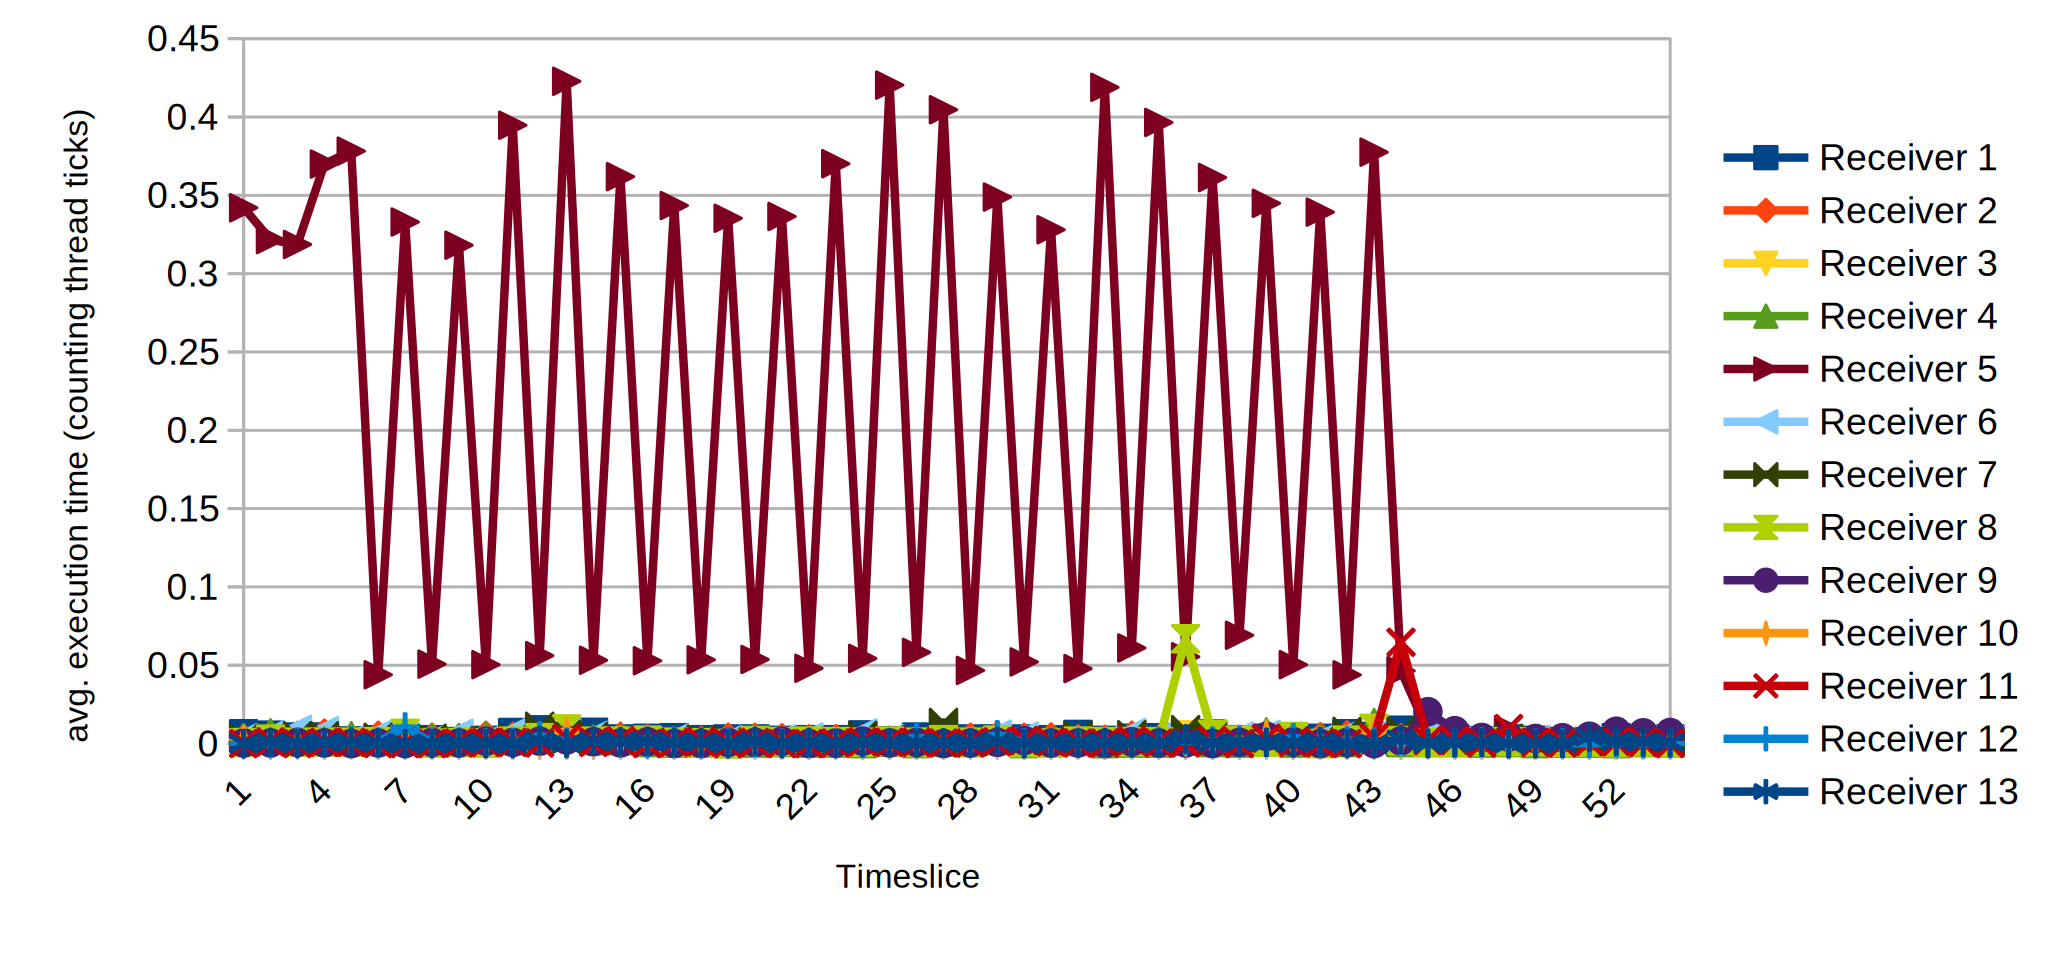
\includegraphics[width=0.75\textwidth]{figures/contentiontest}

    \caption{Average execution time per timeslice (counting thread ticks) during a test run of sending alternating \texttt{0}'s and \texttt{1}'s}
    \label{fig:contentiontest}
    \centering
    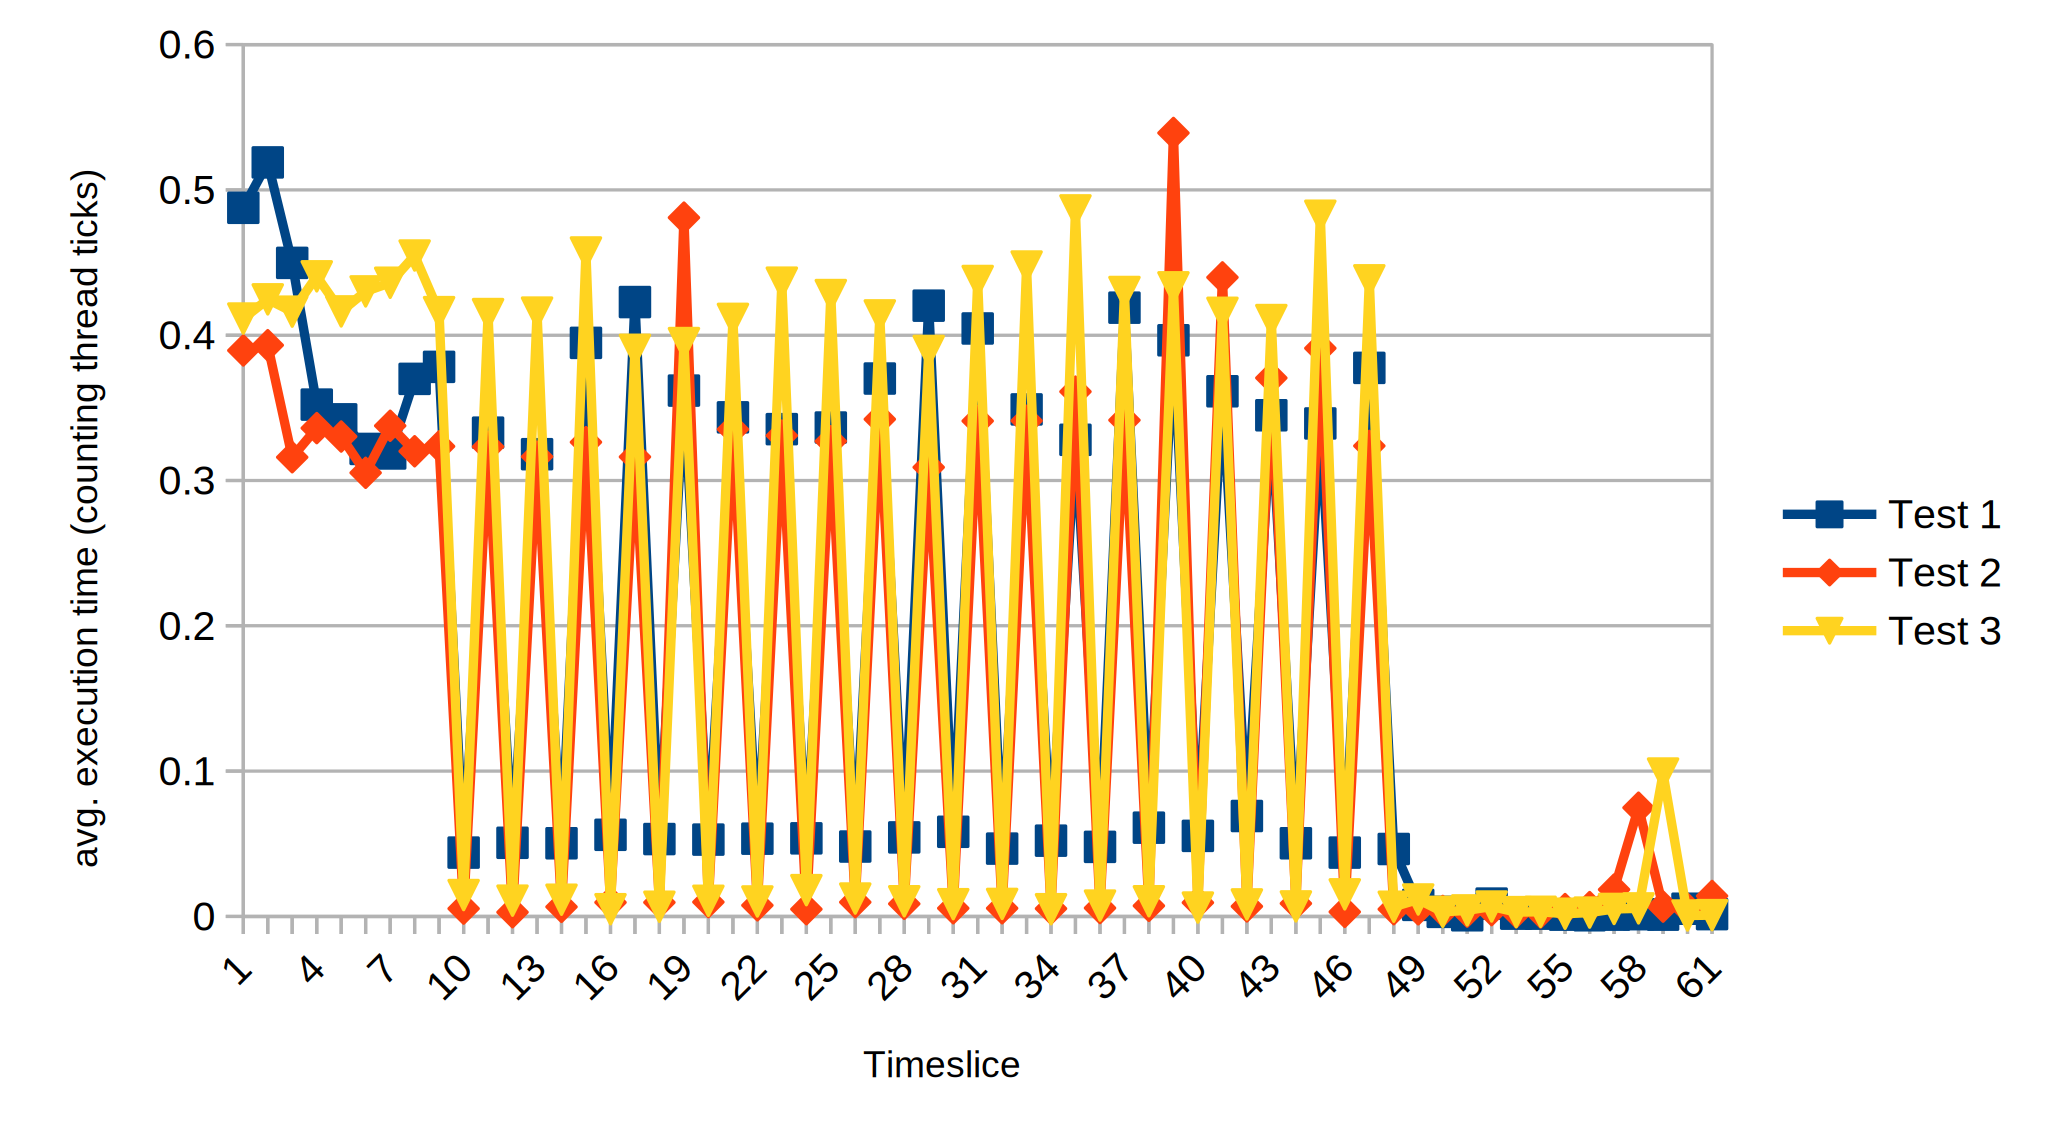
\includegraphics[width=0.75\textwidth]{figures/contentioncoalesced}

    \caption{Average execution time per timeslice (ticks) of the co-located receiver during three test runs of sending alternating \texttt{0}'s and \texttt{1}'s}
    \label{fig:contentioncoalesced}
\end{figure}

Figure~\ref{fig:contentiontest} displays the contention of each receiver for each timeslice.
One can easily see that receiver 5 is co-located with the sender;
it registers alternating high and low contention, in accordance with the alternating \texttt{1}'s and \texttt{0}'s sent by the sender.
Meanwhile, the contention measured by the other receivers stays low.

\section{Targeting a scheduler queue}
JavaSQUIP targets AMD Zen~2, Zen~3 and Zen~4;
these architectures support multiplication only on ALU1~\cite{AMD2020OptimizationEPYC7003}.
When sending a 1, JavaSQUIP makes multiple codependent calls to \texttt{Math.imul()}, which translate to the \texttt{imul} instruction.
This fills up the scheduler queue of ALU1, eventually causing a queue stall.

\begin{lstlisting}[float,caption={The functions \texttt{send\_zero()} and \texttt{send\_one()}},label={lst:sendzeroone},language=JavaScript]
function send_zero(until) {
  until = +until;

  while(+Date.now() < +until) {
    // simply busy waiting
  }
}

function send_one(until) {
  until = +until;

  let i = dummy[0]|0;
  let j = dummy[1]|0;
  while(+Date.now() < until) {
    i = (((i|0) + 100069) % 100103) | 0;
    j = (((j|0) + 997) % 13) | 0;

    // block scheduler queue with 100 imul instructions
    i = Math.imul(i|0, j|0) | 0;
    i = Math.imul(i|0, j|0) | 0;
    // repeats 100 times
    i = Math.imul(i|0, j|0) | 0;
    i = Math.imul(i|0, j|0) | 0;
  }

  // use the result so the calculation is not optimised away
  dummy[1] ^= i|0;
}
\end{lstlisting}

\begin{lstlisting} [float,caption={The squip() function},label={lst:squip}][language=JavaScript]
function squip(start_value, factor) {
  start_value = +start_value;
  factor = factor|0;

  let dummy = +start_value;

  let start_time = Atomics.load(timer, 0)|0;

  dummy = +Math.sqrt(+dummy);
  dummy = +Math.sqrt(+dummy);
  // repeats 10 times
  dummy = +Math.sqrt(+dummy);
  dummy = +Math.sqrt(+dummy);

  dummy = dummy|0;

  dummy = Math.imul(dummy|0, factor|0)|0;
  dummy = Math.imul(dummy|0, factor|0)|0;
  // repeats 20 times
  dummy = Math.imul(dummy|0, factor|0)|0;
  dummy = Math.imul(dummy|0, factor|0)|0;

  let end_time = Atomics.load(timer, 0)|0;

  return {
    dummy: dummy|0,
    time: ((end_time|0) != (start_time|0))|0
  };
}
\end{lstlisting}

In Listing~\ref{lst:sendzeroone} and Listing~\ref{lst:squip}, many features of the JavaScript environment are utilised to ensure the correct behavior of the program.
The most noticeable is the use of \texttt{|0} for many operations with numbers.
It forces the interpretation of the given constant or variable as an integer, thus simplifying the operation.
For example, \texttt{1.4|0 + 4.5|0} will be interpreted as an integer addition and evaluate to \texttt{5}. \\
Similarly, using a variable with a~\texttt{+} in front -- as in line 2 -- will force a reinterpretation as a floating-point number.
We use \texttt{Atomics.load()}~\cite{atomicsload} to get the current value of the counting thread.
It is an atomic operation, so thread safety and correctness of the value are ensured.

The codependence of the \texttt{imul} operations ensures that they have to be executed one after the other, in order.
It is ensured simply by using the result of one operation as the input for the next.
The input for the \texttt{imul} operations is calculated in lines $15$ and $16$ of Listing~\ref{lst:sendzeroone} based on an input variable \texttt{dummy}.
This prevents the JIT-compiler from pre-computing the result and optimizing away the \texttt{imul} calls.


Listing~\ref{lst:sendzeroone} shows two functions of the sending process.
The functions are for sending a zero or a one respectively, in a given time frame.
The parameter \texttt{until} gives the end of the timeslice to send a bit.

\section{Detecting scheduler queue contention}
\label{sec:detect-sqc}
The receiving process needs to detect whether the sender has sent a \texttt{1} or a \texttt{0}.
This is equivalent to detecting scheduler queue contention.
This is implemented by issuing several \texttt{imul} instructions,
and measuring the delay with the help of a separate counting thread.

Listing~\ref{lst:squip} shows how the receiver issues 10 \texttt{sqrt} and 20 \texttt{imul} instructions,
retreiving the counter value before and after (see lines \texttt{7} and \texttt{23}).
If the retire control unit is not blocked by an overflowing scheduler queue,
the instructions can be reordered so both reads of the counting value are right after one another.
This results in the measured time delay being zero, which means no scheduler queue contention took place.
If the two values are not equal, we can deduce that the program flow was held up by scheduler queue contention:
The program flow was not reordered because the scheduler was stalled, and the counting thread increased the counter
between the execution of line \texttt{7} and line \texttt{23}.

The combination of \texttt{sqrt} and \texttt{imul} instructions is selected because they work on different scheduler queues.
If the scheduler queue for ALU1 overflows because of the additional \texttt{imul} instructions,
the whole instruction queue stalls -- which prevents the reordering of lines \texttt{7} and \texttt{23}.
In this case, the \texttt{sqrt} instructions are also stalled, further increasing the execution time between lines \texttt{7} and \texttt{23}.
In the case that no stall occurs, the additional \texttt{sqrt} instructions do not hinder the program flow,
since they target a different scheduler queue.

In line \texttt{27}, that we do not check the actual difference between \texttt{start\_time} and \texttt{end\_time},
but rather only return a \texttt{1} if the two are different, and a \texttt{0} otherwise.
Since we can assume that a difference in \texttt{start\_time} and \texttt{end\_time} is an indicator of scheduler queue contention,
this gives a good measurement;
a \texttt{0} is returned when there is no contention, and longer execution times do not throw off the average,
since at maximum a \texttt{1} can be returned.
Returning the actual difference of the counting thread values, i.e. returning the actual execution time, mostly gives equal results.
Some measurements are however thrown off by longer delays in execution,
which increases the average execution time unproportionally.

The \texttt{squip} function is run 100 times per timeslice, summing up the return values of each iteration.
At the end of the timeslice, this sum is divided by 100,
resulting in the relative likelihood of a queue stall between time measurements, or \textit{stall likelihood}.
If the stall likelihood is above the threshold (see Section~\ref{sec:delaythreshold}), a \texttt{1} is registered, else a \texttt{0}.
Figure~\ref{fig:contentioncoalesced} shows that scheduler queue contention usually affects around $30-50~\%$ of the tries in a timeslice.
Since this metric is closely related to the execution time of the measurement, the two terms are used interchangeably in the rest of this thesis.


%--- OPTIMISATION --------------------------------------------------------------
\chapter{Optimisation}
\label{ch:optimisation}
\begin{figure}
\centering
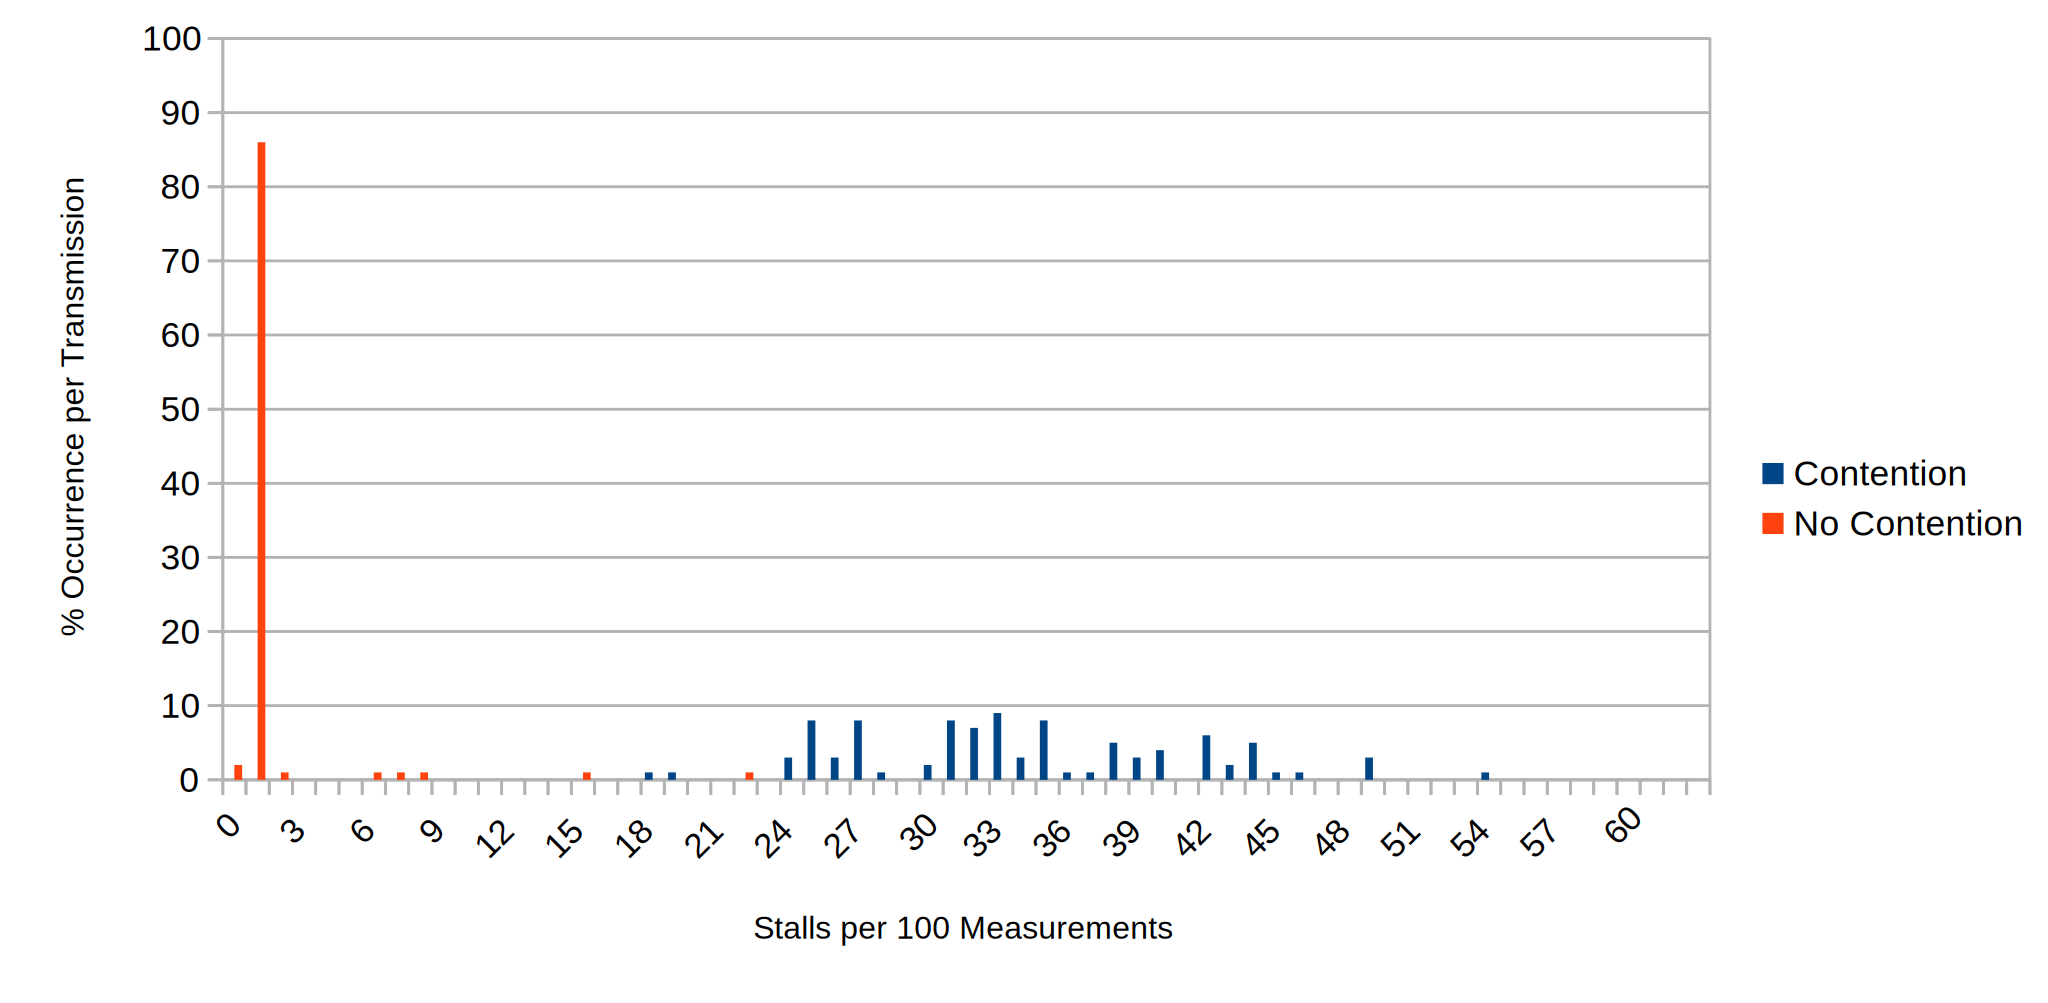
\includegraphics[width=0.9\textwidth]{figures/contentionhistogram}

\caption{Distribution of stall likelihood per timeslice with and without scheduler queue contention by the sender}
\label{fig:contentionhistogram}
\end{figure}

JavaSQUIP is intended to show SQUIP's potential as an attack in a browser setting.
Because of this, we aim to make it as fast and stable as possible.
The transmission speed is limited by the environment, as the time slices cannot be smaller than 1ms.
The remaining settings and features are adjusted so the transmission is as accurate as possible at the speed of 1000 bits/s.

\section{Delay threshold}
\label{sec:delaythreshold}

The simplest parameter in SQUIP is the delay threshold.
It determines whether the summed up delay of a timeslice is registered as a \texttt{0} or a \texttt{1}.
If the threshold is too high or too low, results are skewed towards registering a \texttt{0} or a \texttt{1} respectively.

To tune this parameter, the resulting bitstream is checked against the actual sent stream.
All of the bits that are wrongly registered as \texttt{1} or wrongly \texttt{0} are tallied up separately.
Then the delay threshold is adjusted until faulty \texttt{1}'s and faulty \texttt{0}'s are approximately equally frequent,
meaning that no skew toward high or low bits is present and the delay threshold is set optimally.

Figure~\ref{fig:contentionhistogram} shows the distribution of execution times per timeslice with and without scheduler queue contention.
Timeslices without scheduler queue contention show very short execution times, except for a small number of outliers.
Execution times for timeslices with scheduler queue contention vary more, though they are clearly separable from those without contention.
A threshold value of $0.21$ is optimal, giving the best margin for \texttt{0}- and \texttt{1}-transmissions.


\section{Number of instructions for a queue stall}
The sender blocks a targeted scheduler queue by sending a large number of instructions to it.
The number of instructions is another tunable parameter:
it needs to be big enough to cause a queue stall and a spike in execution time,
yet it needs to be as small as possible to minimise chance of a stall bleeding into the following timeslice.

To tune the number of \texttt{imul} instructions, a bleed-over test is constructed.
It test consists of a string of alternating \texttt{1}s and \texttt{0}s, so contrasts between different bits could be easily observed.
The amount of \texttt{imul} instructions is tuned by successively reducing the number and running a test.
The point where no spike in execution time is registered any more is set as the lower limit for the amount of \texttt{imul} instructions.
Figure~\ref{fig:contentiontest} shows the final tuned system;
the spikes for a \texttt{1} are pronounced, while the execution time in a \texttt{0}-timeslice is only slightly higher than for the remaining receivers.
For Zen~4 systems, 200 co-dependent \texttt{imul} instructions are the optimum.
Small changes to the number of instructions do not create meaningful differences in performance.
Figure~\ref{fig:contentioncoalesced} illustrates that this system is quite robust across different tests.

\section{Minimising contention by the receivers}
\label{sec:reducecontention}
The receiver detects a queue stall by measuring whether two operations were reordered to be right after one another,
or whether the scheduler queue was stalled between the two operations by contention.
To detect a stall, the execution time for \texttt{imul} instruction calls is measured.
See Section~\ref{sec:detect-sqc} for a detailed explanation of the stall detection.

To improve the signal-to-noise ratio, the receivers should create as little contention as possible themselves.
This is helpful in the transmission, as it reduces the contention for two co-located receivers,
maximizing the contrast to the receiver that is co-located with the sender (see \ref{sec:co-location})
Three optimisations are employed in the receiver worker: adjusting the \textit{number of stall instructions},
using \textit{buffer instructions}, and a \textit{delay loop}.

\paragraph{Number of stall instructions.}
To get a more stable result, several successive \texttt{imul} instructions are used.
On the other hand, too many instructions would create contention themselves, so fewer instructions would be better.
A detection test is set up to determine the minimum amount of instructions to be able to detect contention by the sender.

The detection test is constructed similarly to the bleed-over test:
alternating \texttt{1}s and \texttt{0}s are received, and the delays measured.
The number of \texttt{imul} instructions in the receiver worker is reduced until no signal is retrievable,
resulting in a lower bound for the number of \texttt{imul} instructions in the receiver worker.
For Zen~4, the optimum number of \texttt{imul} instructions is $20$.

\paragraph{Buffer instructions.}
In the measurement function, 10 \texttt{sqrt} instructions serve as a buffer to delay the \texttt{imul} instrucions:
they delay the execution, while not creating contention on ALU1.
This means that the effect of a stalled queue is more pronounced, because the \texttt{sqrt} instructions will also be stalled.
On the other hand, they have little effect on an unstalled queue, since they operate on a different scheduler.
The implementation can be seen in Section~\ref{sec:detect-sqc}

\paragraph{Delay loop.}
\begin{lstlisting}[float,caption={The delay loop after a measurement},label={lst:delayloop},language=JavaScript]
let k = 0|0;
while(k < 1000|0) {
  dummy  ^= k|0;
  k += 1;
}
\end{lstlisting}

A delay loop is added after each measurement to clearly separate measurements.
To this effect, we fill the scheduler queue with other operations for a short time between measurements.
Since no normal delay function gives a better accuracy than 1ms, a busy-waiting loop is used.
Listing~\ref{lst:delayloop} shows the delay loop that is executed after each measurement.


Figure~\ref{fig:contentiontest} demonstrates these measures working:
Receiver 5 -- which is co-located with the sender -- receives a clean signal of alternating \texttt{1}'s and \texttt{0}'s.
Meanwhile, all the remaining receivers -- which are co-located either with each other or with the counting thread -- show very little contention.


%--- EVALUATING JAVASQUIP --------------------------------------------------------------
\chapter{Evaluating JavaSQUIP}
\label{ch:evaluation}

To evaluate and measure different parameters and settings, we set up a test scenario for JavaSQUIP.
It consists of two web pages communicating with each other solely over the JavaSQUIP covert channel.

\section {Test setup}
\label{sec:testsetup}
To evaluate JavaSQUIP on both the Zen~3 and Zen~4 architecture,
we test on an \textit{AMD Ryzen 7 5800X} as representative for Zen~3 and an \textit{AMD Ryzen 7 7700X} as representative for Zen~4.

The test setup consists of two webpages: a sender and a receiver.
The sender simulates the target, and the receiver simulates a page that is controlled by the attacker.
Because the attacker has little or no control over the target, we keep the sender page minimal.
The sender has only one working thread.
The working thread is sending either a 0 (no action) or a 1 (contention with codependent \texttt{Math.imul()} calls) for each timeslice.
With more control over the receiver, the attacker can ensure co-location from this side.
For our tests on the \textit{AMD Ryzen 7 5800X}(Zen~3) and \textit{AMD Ryzen 7 7700X}(Zen~4), we need 14 receiving workers.
An explanation for the number of receivers needed can be found in Chapter~\ref{sec:co-location}.

To distinguish a message from random noise on the CPU, the sender sends a preamble before the actual data.
The preamble is a sequence of the numbers from 100 through 109.
If the receiver sees two ascending bytes between 100 and 109, it is highly likely that this is part of the preamble --
a message was detected.
For easier evaluation of the transmission accuracy, the message is also stored on the receiver's side,
so that the number of "faulty \texttt{1}" and "faulty \texttt{0}" bits can be automatically calculated.
In our test setup, messages of 500 random bytes are sent at a transmission speed of 1000bits/s.
This results in a transmission time of $\frac{500 \times 8}{1000} = 4$ seconds.

\section{Speed}
The sender and receiver need to know the desired transmission speed beforehand to match up their timeslices.
This means that the transmission speed is a fixed value and needs no further calculation.
Due to the reduced resolution of the Date.now() timer used for the time slices (see Section~\ref{sec:accurate-timing}),
our best achievable speed is 1000bits/s.

There is, however, still some overhead for the preamble (see Section~\ref{sec:testsetup}).
It is a fixed size of 10 bytes regardless of the message,
so the relative overhead tends to $0~\%$ as the message size increases.

\section{Reliability}
There are two aspects that affect the reliability of the covert channel:
First, the sender being co-located with a receiver, and second, the resilience of the covert channel against noise.

\paragraph{Co-location.}
To measure the actual co-location probability, we use preamble system as described in Section~\ref{sec:testsetup}.
Threads are unlikely to be relocated during the 4 seconds of a transmission,
and the preamble is likely to be recognised if co-location is given (see noise resilience further down).
We can conclude that the rate of recognised preambles is a good measurement for the actual co-location probability.

In our tests, we find an average co-location probability of $88.7~\%$ in a Zen~3 architecture and $96~\%$ in Zen~4.
This is consistent with the theoretical co-location probability of $93.3~\%$ calculated in Section~\ref{sec:co-location}.

When tested under stress with \texttt{stress --cpu 1}, we achieve an average co-location probability of $53.7~\%$.
Most likely, the sender is co-located to a receiver more often than that,
but the corresponding receiver is not able to detect the preamble due to the noise.
When run simultaneously with \texttt{stress --cpu 2}, JavaSQUIP is not able to receive the preamble.
As a result, co-location is never detected and transmission of data is not possible.

\begin{figure}
    \centering
    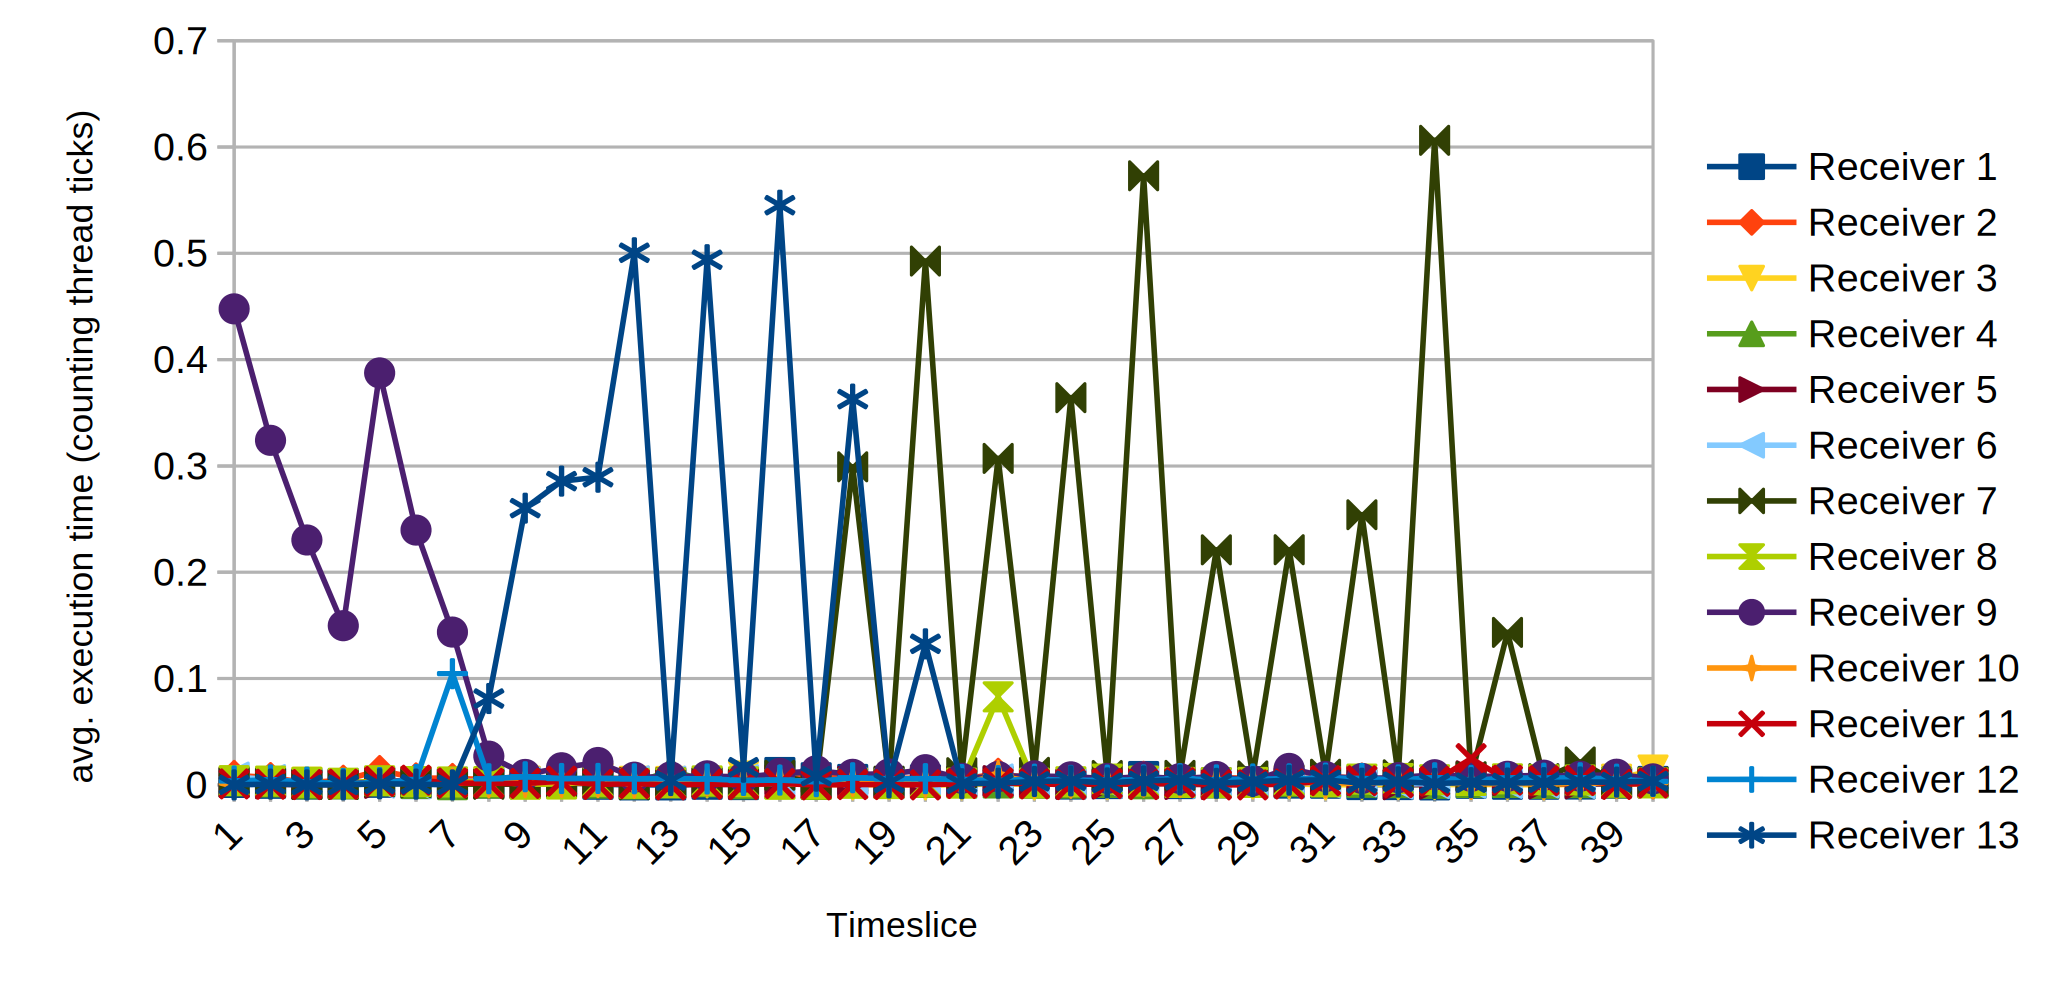
\includegraphics[width=0.75\textwidth]{figures/contentiontest_stress}

    \caption{Execution time per timeslice during a test run of sending alternating \texttt{0}'s and \texttt{1}'s with \texttt{stress --cpu 1}}
    \label{fig:contentiontest_stress}
\end{figure}

\paragraph{Noise.}
For measuring noise resistance, we only take into account those transmissions where the preamble was recognised.
This results in an average transmission accuracy of $99.2~\%$ on Zen~3, and $99.3~\%$ on Zen~4.
With \texttt{stress --cpu 1}, we observed an accuracy of $74~\%$.

\ref{fig:contentiontest_stress} shows the effect of outside CPU stress on the measurement.
Although the \texttt{stress} command creates more noise in the measurement, the overall contention levels go down (compare with \ref{fig:contentiontest}).
This is because \texttt{stress} does not target a specific scheduler queue, but instead takes up CPU time with a varied set of instructions.
The result is more relocation of threads (the sending thread is first co-located with receiver 13, later with receiver 7), and less contention.

\paragraph{Effective transmission rate.}
We define the \textit{effective transmission rate} as the rate of correctly received bits.
For example, a transmission at 2000~bits/s with an error rate of 10~\%
has an effective transmission rate of 1800~bits/s:
\[2000~\text{bits/s}~*~(100~\%~-~10~\%)~=~1800~\text{bits/s}\]

The effective transmission rate may differ from the usable bandwidth of the covert channel,
depending on the transmission protocol and error correction.
Nevertheless, it gives a good estimate to compare usable bandwidth between different covert channels.

For JavaSQUIP, we take into account both the co-location probability and the transmission accuracy.
By multiplying these values, we calculate an effective transmission rate of 880~bits/s on Zen~3:
\[1000~\text{bits/s} * 88.7~\% * 99.2~\% \approx 880~\text{bits/s}\]
The effective transmission rate on Zen~4 is 986~bits/s:
\[1000~\text{bits/s} * 93.3~\% * 99.3~\% \approx 986~\text{bits/s}\]

%--- COMPARISON ----------------------------------------------------------------
\chapter{Comparison to other browser covert channels}
\label{ch:comparison}
We have shown that JavaSQUIP is a fast and robust cross-instance covert channel for modern browsers.
To further illustrate the power of JavaSQUIP,
we will now compare its performance to similar modern browser-based covert channels.
For a fair comparison, they need to exhibit data transfer between browser instances,
with all the current security mitigations in place (see Section~\ref{sec:browsersecurity}).
The selected covert channels are the following:

\begin{itemize}
    \item \textit{Event Loops}~\cite{vila2017loophole}
    \item \textit{Hardware Interrupts}~\cite{lipp2017practical}
    \item \textit{Port Contention}~\cite{Rokicki2022webport}
\end{itemize}

As browser-based timing covert channels, they share a few common traits.
All of them need a way to create contention and a way to measure it.
The common solution is with a sender that either idles or performs an action,
while the receiver continually monitors the execution time of a loop that is sensitive to this action.

\section{Event Loops}
The \textit{Loophole} Timing Attack~\cite{vila2017loophole} uses shared event loops to get timing information.
An Event loop is a piece of code that continually checks for an event condition
and starts registered event handlers if the event has occurred.
An example would be an event loop that checked for a \textit{Space} key press,
which starts an event handler to start a video on the website.

The version of the covert channel attack we are interested in relies on two pages sharing the same \textit{renderer process}.
The renderer process takes care of the parsing, execution, and rendering of the JavaScript sandbox.
Consequently, pages in the same renderer process also share resources more closely.
This is used to get access to shared event loops with more accurate timing information.

The following ways of sharing a renderer process have been found:

\begin{itemize}
    \item embedding in an Iframe
    \item creation of the new page by the renderer, e.g. through a link-click, or scripted redirect
    \item reuse of renderers by Chrome for resource optimisation
\end{itemize}

Having one of these is possible, though it does limit the applicability of this covert channel.
The authors of the paper also presented a version of the covert channel that works without a shared renderer process,
at the cost of a significant decrease in transmission rate.

Vila et al. proposed a covert channel where the receiver continually checks the delay of an event handler
that is triggered by a shared event loop.
With a shared renderer process, they achieved a transmission speed of \textbf{200 bits/s}.
Their solution without a shared renderer process ran at a transmission speed of only \textbf{5 bits/s}.
Vila et al. did not discuss the error rate of transmissions in their paper.

\section{Hardware Interrupts}
In their paper on \textit{Practical Keystroke Timing Attacks in Sandboxed JavaScript}~\cite{lipp2017practical},
Lipp et al. explored a side channel based on hardware interrupts.
To get information about a hardware interrupt being triggered,
a script continually requests and logs the time increase of \texttt{performance.now()}~\cite{performancenow}.
If this script is preempted by a hardware interrupt (e.g. for a keystroke),
the delta to the last measured timestamp is significantly higher.
This allows the attacker to infer that a hardware interrupt was triggered.

To convert this side channel into a covert channel,
the researchers needed a hardware interrupt that the sending web page could trigger.
They found that issuing an \texttt{XMLHttpRequest} to an invalid site would cause an I/O interrupt.
The sender would now issue these requests to send a \texttt{1} and remain idle to send a \texttt{0}.
The receiver measures the bits the same way as described above --
by continually looking up the value of \texttt{performance.now()}.

This hardware interrupt-based covert channel has no notable limitations:
It works in a cross-browser setting on a wide range of devices and processors.
With time slices of 40ms length, the resulting transmission speed is \textbf{25 bits/s}.
Lipp et al. did not share the error rate of their covert channel.

\section{Port Contention}
The principle of port contention is the most similar to JavaSQUIP's scheduler queue contention.
The receiver runs a loop of issuing an instruction on a particular port and measures its execution time.
Whenever the sender issues an instruction on the same port, the receiver's instructions on that port take longer,
thus delaying the measurement loop.

In \textit{Port Contention Goes Portable}~\cite{Rokicki2022webport},
Rokicki et al. showcased a feasible application of port contention in a browser-based covert channel.
As opposed to the 1-sender multi-receiver approach of JavaSQUIP (see Section~\ref{sec:general-architecture} and Section~\ref{sec:co-location}),
their solution features 1 receiver and multiple senders.
The measurement loop of the receiver was implemented in \textit{WebAssembly} to easily issue a particular instruction.
Since the single receiver is sandboxed in JavaScript, it can neither bind to a physical core, nor know which core it is on.
Consequently, the sender creates as many threads as there are cores on the machine.
The sender was implemented as a native program running unprivileged code.
This still gave the researchers the opportunity to bind each thread to a different core,
ensuring that one of them would be co-located with the receiver.

Rokicki et al. discussed the possibility of altering their covert channel to be fully within two browser instances.
They proposed a similar solution to the problem of co-location as the one we have implemented for JavaSQUIP.
On this basis, they believably argued that this fully web-based attack would have the same transaction speed as the version
with a native sender at \textbf{200 bits/s}.
They reported a packet loss rate of 5.5~\% and an error rate of 1~\%.
The resulting effective transmission rate is \textbf{187 bits/s}:
\[200~\text{bits/s} * (100~\% - 5.5~\% - 1~\%) = 187~\text{bits/s}\]

\section{Feasibility of JavaSQUIP}

%\begin{figure}
%\centering
%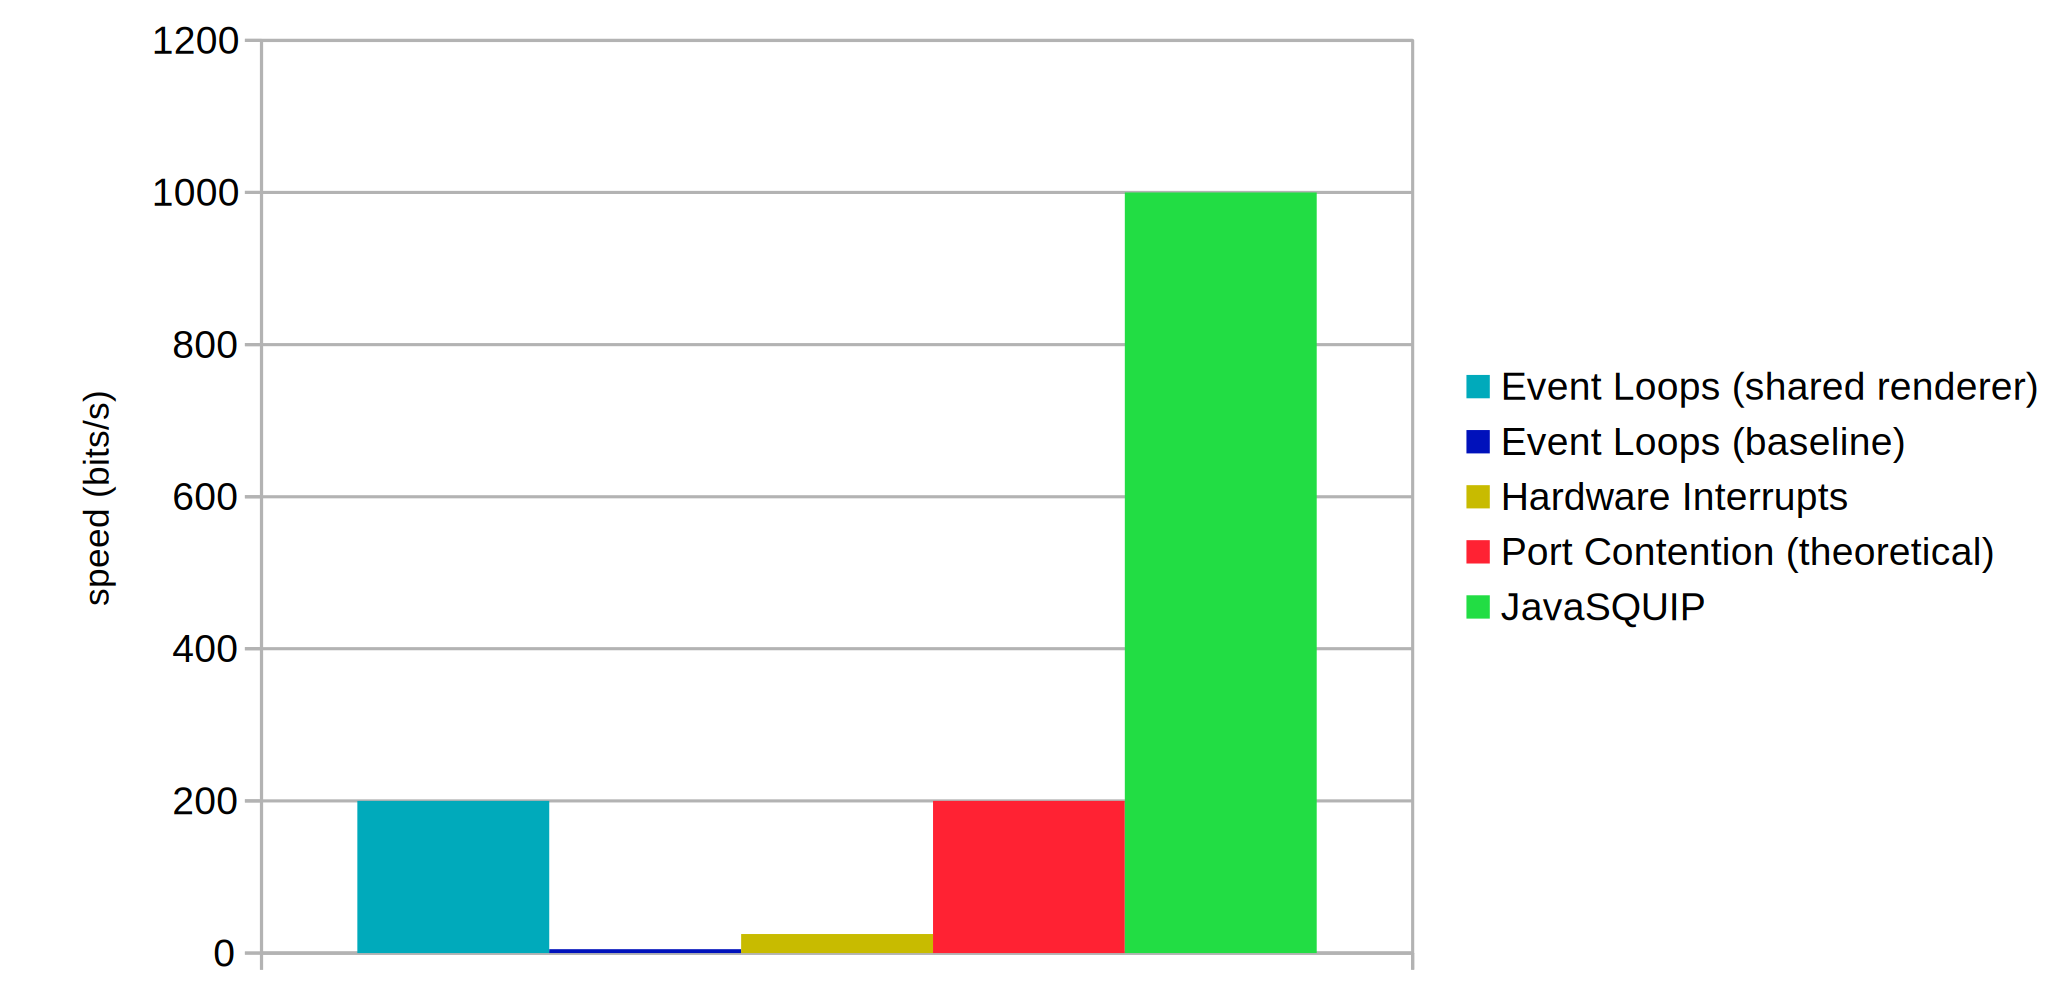
\includegraphics[width=0.8\textwidth]{figures/speedcomparison}
%\caption{A comparison of transmission speeds between browser-based covert channels.}
%\label{fig:speedcomparison}
%\end{figure}

\begin{table}[t]
\centering
\begin{tabular}{ |l|r|r| }
\hline
\textbf{Covert channel} & \textbf{theoretical speed} & \textbf{effective speed} \\
\Xhline{2pt}
Event Loops (shared renderer) & 200 bits/s & ? \\
\hline
Event Loops & 5 bits/s & ? \\
\hline
Hardware Interrupts & 25 bits/s & ? \\
\hline
Port Contention & 200 bits/s & 187 bits/s \\
\hline
JavaSQUIP(Zen 3) & 1000 bits/s & 880 bits/s\\
\hline
JavaSQUIP(Zen 4) & 1000 bits/s & 986 bits/s\\
\hline
\end{tabular}

\caption{A comparison of transmission speeds between browser-based covert channels.}
\label{tab:speedcomparison}
\end{table}

\paragraph{Affected CPUs.}
JavaSQUIP exploits a vulnerability in the split-scheduler design of AMD's Zen~2, Zen~3 and Zen~4 architectures.
This means that JavaSQUIP only works on clients running on a CPU with one of these architectures.
This limits the attack surface significantly, though the number of affected computers is still significant.
As of Q3 of 2024, AMD holds a market share of around $33~\%$ in CPUs~\cite{amdmarket}.
Most of these CPUs run under the Zen~2, Zen~3 and Zen~4 architecture,
meaning that large portion of current computers is susceptible to this attack.

\paragraph{Website prerequisites.}
Some of the above-mentioned covert channels need a particular environment in the browser to mount the attack.
The \textit{Loophole} covert channel needs a shared renderer process.
While the port contention approach can theoretically work without a native sender,
the receiver still requires \textit{WebAssembly} support to work.

JavaSQUIP on the other hand has none of these limitations.
The covert channel can be established on any two browser instances where normal JavaScript can be run.
Other than \texttt{Date.now()}~\cite{datenow} and \texttt{SharedArrayBuffer}~\cite{sharedarraybuffer},
no higher-level APIs are needed.
As an example, even two malicious adverts on different browser instances could conceivably communicate with each other
with JavaSQUIP.

\paragraph{Speed.}
JavaSQUIP transmits data at a speed that is currently unmatched by any covert channel in a browser with up-to-date security settings.
Its theoretical transmission capacity is \textbf{1000 bits/s}.
We observed an effective transmission speed of \textbf{880 bits/s} and \textbf{986 bits/s} for Zen~3 and Zen~4 respectively.
This is enough bandwidth to support a live transmission of all user inputs, or to transmit a short audio recording within minutes.
JavaSQUIP's effective transmission speed surpasses the theoretical speed of all other covert channels mentioned in this chapter at least by a factor of 4.

%--- CONCLUSION ----------------------------------------------------------------
\chapter{Discussion of Countermeasures}
\label{ch:countermeasures}

The preceding chapters have shown that JavaSQUIP is a powerful covert channel.
We want to discuss several ways to impede or prevent the usage of this vulnerability for nefarious purposes.
First, we will discuss possibilites to alter the three features needed to implement JavaSQUIP:
\textit{timing functions}, \textit{multithreading}, and \textit{low-level operations}.
We finish by discussing more ways of \textit{preventing co-location} of the sender and receiver.

\section{Timing functions}
JavaSQUIP uses two timers: \texttt{Date.now()}~\cite{datenow} and a counting thread (see Section~\ref{sec:accurate-timing}).
The counting thread is based on multithreading, which will be discussed in the next section.

The resolution of \texttt{Date.now()} directly affects the available transmission speed.
The usefulness of JavaSQUIP can be easily decreased by decreasing the time resolution.
On the other hand, going below 1 ms-accuracy would make the feature too weak.
Many legitimate programs need this accuracy in timing measurements,
for example for performance assessments of a website.

Even if the resolution of \texttt{Date.now()} was reduced,
the covert channel would still be able to synchronize clocks between sender and receiver.
Thus, there is no feasible way to counteract the JavaSQUIP attack by decreasing timer accuracy.

\section{Multithreading}
Removing the support for \texttt{Web Workers}~\cite{webworkers} or a \texttt{SharedArrayBuffer}~\cite{sharedarraybuffer}
would break JavaSQUIP.
Obviously, disabling these features outright is not a satisfactory solution.
It would force every website to run all code in the main thread,
drastically reducing responsiveness for websites with bigger computational needs.

One possibility would be that browsers provide a way to disable access to these resources on a \textit{per-site} or a \textit{per-script} basis.

With \textit{per-site} restriction of \texttt{Web Workers}, a user could prevent an untrusted website from implementing JavaSQUIP.
It is not reasonable to ask the user's permission to this widely used API,
so only a blacklist by the user would be feasible.
Most users would likely not use this feature, making it generally ineffective.

A \textit{per-script} permission system could give a benign website the option to load scripts from an untrusted source (e.g. third-party advertisements),
running them with constrained permissions.
This way, the host website could still make use of the multithreading features while preventing a JavaSQUIP attack by third-party scripts.
Because there is no ad-hoc way for the browser to tell a trusted script from an untrusted one,
website developers would have to explicitly give the information to the browser not to trust a script.
Again, this mitigation would most likely lose its effect due to not being used.

\section{Low-level operations in JavaScript}
JavaSQUIP targets ALU1 with \texttt{imul} instructions using \texttt{Math.imul}~\cite{mathimul}.
Browser providers could disable this API call without affecting too many websites,
but there are simple workarounds for this.

WebAssembly~\cite{webassembly} is currently supported in all major browser engines.
It promises to provide web developers with faster execution times by circumventing JavaScript's just-in-time compiler.
Pre-compiled WebAssembly binaries can be executed directly in the browser.

JavaSQUIP could easily be implemented in WebAssembly, using its fine-grained control over instructions to
target a scheduler queue.
WebAssembly is currently a rising technology -- more and more websites are implementing it~\cite{musch2019new}.
It is unlikely that browser developers are going to disable support for it.
Consequently, there is currently no way to prevent a website from targeting a scheduler queue.

\section{Preventing co-location}
Because JavaSQUIP depends on co-location of the sender and one of the receivers,
preventing co-location would present a way to make the covert channel impossible.
The simplest way would be to disable simultaneous multithreading,
though few users will accept this because of the performance loss of about $25~\%$~\cite{Phoronix2018HT, Cutress2020SMT}).

Process-based separation of physical CPU cores also works to mitigate the vulnerability.
This approach still makes use of SMT, but prevents threads of different processes to be co-located.
This way, multi-threaded programs (and in extension websites) can still benefit from the technology,
while SMT-based side channels are fundamentally prevented.
SMT-COP~\cite{townley2019smt} expands on this idea.
This would have to be implemented at the scheduler level, requiring an operating system-level update.
Similar to the security update to mitigate Spectre~\cite{spKocherHFGGHHLM019},
this update would have a negative impact on the computer's overall performance.
Implementing SMT-COP results in a performance loss of 4~\% to 10~\%, depending on the workload.

%--- CONCLUSION ----------------------------------------------------------------
\chapter{Conclusion}
\label{ch:conclusion}
In this thesis, we ported the SQUIP~\cite{squip} attack to a JavaScript context, thus creating the JavaSQUIP covert channel.
JavaSQUIP has achieved a transmission rate of 1000 bits/s, showing an advantage in performance over
all other current JavaScript-based covert channels~\cite{vila2017loophole, lipp2017practical},
in particular over attacking single-scheduler based architectures~\cite{Rokicki2022webport}.

Additionally, we observed a co-location rate of $88.7~\%$/$96~\%$ with a transmission accuracy of $99.2~\%$/$99.3~\%$ (Zen~3/Zen~4).
This shows that architectures with multiple scheduler queues present a bigger attack surface than their single-scheduler counterparts.

JavaSQUIP breaks the sandboxing model of a web browser context.
This means that one browser instance can communicate with another without using the network, thus being virtually undetectable for an unknowing victim.
This could potentially be used by malicious code within a website -- no matter its origin -- to exfiltrate data to another browser instance on the same computer.
Its speed and accuracy enable an attacker to transmit large amounts of data, such as images or short audio clips, within the lifetime of a malicious web page.

Though security updates in modern browsers slow down and hinder timing attacks, microarchitectural attacks have not yet been eliminated.
JavaSQUIP mostly uses JavaScript features that have already been restricted to improve security as much as feasible;
mitigating microarchitectural attacks in a browser setting proves to be increasingly hard as CPUs grow more and more complex.
We have shown that there are few options for counteracting JavaSQUIP and similar attacks.
All of the solutions proposed in this paper have requirements that make them unlikely to be implemented.
Thus, we can expect JavaSQUIP -- along with many other browser-based covert channels --
to remain viable for the near future.

%--- BIBLIOGRAPHY --------------------------------------------------------------
\pagebreak
\printbibliography

\end{document}
